\section{Introduction}
Answering questions that require reasoning over a long sequence, such over long documents or multiple documents, is a challenging task~\cite{quality2021}. 
Research in this domain mostly includes tasks that involve multiple text segments, over benchmarks like HotpotQA~\cite{yang-etal-2018-hotpotqa} and QAsper \cite{dasigi-etal-2021-dataset}. 
HotpotQA is a multi-hop QA benchmark over multiple paragraphs from Wikipedia, while QAsper involves reading comprehension from long academic papers, where relevant information on a question could be spread across the paper. 

Given the task complexity \cite{choi-etal-2017-coarse}, benchmarks often provide an additional set of evidence spans, such as sentences or paragraphs, for a given question answer pair. 
This breaks down the long-context QA task, adding a preliminary evidence span detection, which is crucial for successfully finding the correct answer, and also potentially helps in model interpretability. In this work, we propose a method for improving long-context QA via leveraging such evidence spans, by maximizing their similarity with the question.


Since identifying the evidences provides relevant information for answering the question, prior work showed that jointly training models to perform evidence span extraction in addition to answer generation is important for achieving high performance \cite{yang-etal-2018-hotpotqa,dasigi-etal-2021-dataset}. 
To jointly perform evidence extraction and question answering, models utilize sentence representations (marker tokens) in the input; the final layer representation corresponding to these markers is then passed through a classification layer and is optimized using the cross-entropy loss in conjunction with the answer extraction/generation loss. We conjecture and demonstrate (see Table~\ref{tab:map}) that this objective does not sufficiently capture relationships between the question and the candidate evidence spans. Thus, we propose a complementary objective for enforcing question-evidence \textit{similarity} in the model representation (see~Fig.~\ref{fig:model}). Further, we show that optimizing the question-evidence similarity under a certain subspace by using linear projection of the raw representations may softly impose information encoding about their relatedness. Since questions may be partitioned into several types (e.g., yes/no, generative, non answerable, etc.) in the common QA settings, we also investigate learning separate projections per question type.

\begin{figure*}
\centering
  \centering
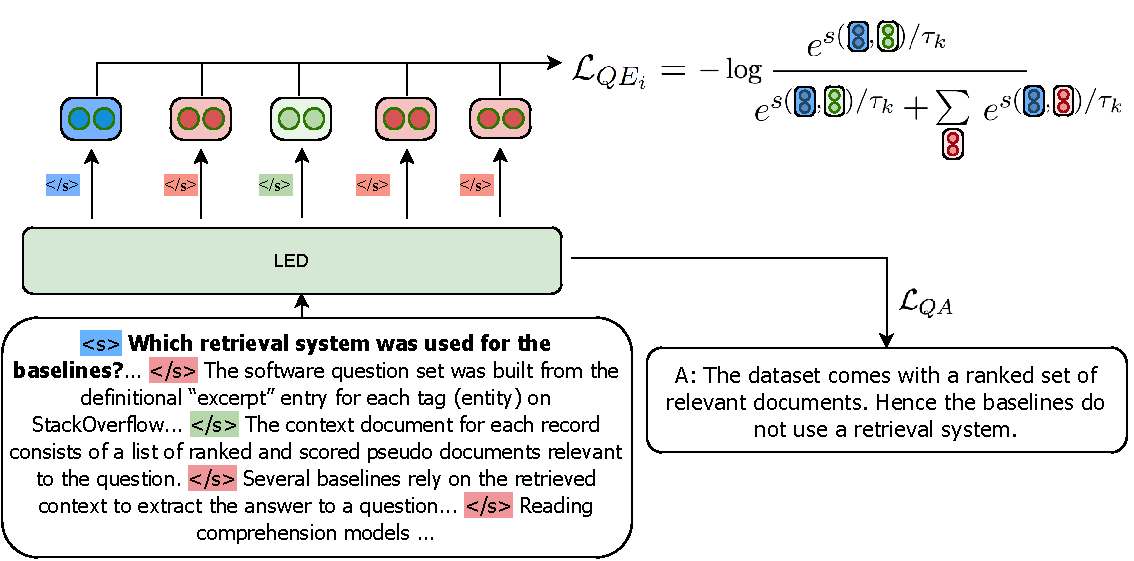
\includegraphics[width=0.99\linewidth]{figures/fig2.pdf}
\caption{Demonstration of our method over an example instance from QAsper~\cite{dasigi-etal-2021-dataset}. A long sequence is fed to a model, producing representations for the marker special tokens. Then, these vectors are used to compute our contrastive objective. The token colored in blue represents the question, and the tokens colored in green (red) represent positive (negative) evidence sentences. The goal is to maximize the similarity between the blue vector and the green vectors.}
\label{fig:model}
\end{figure*}





Driven by the intuition that questions should be similar to their supporting evidences, under some specific geometric sub-space, we propose a novel supervised contrastive learning objective for the finetuning stage, aiming to maximize similarity of question-evidence representations. Contrastive learning has been recently applied to a variety of deep learning models in computer vision \cite{chen2020simple, chen2021exploring} and NLP~\cite{gao-etal-2021-simcse,gunel2021supervised}. Unlike prior NLP related methods, our proposed loss term is model-agnostic and operates in the \textit{sequence-level} in a supervised manner. This objective targets question and evidence representations within input sequences, and unlike prior work, it is not based on individually encoding sentences or paragraphs.  We show that our additional contrastive supervision provides consistent improvements on three different models and two datasets, demonstrating its effectiveness and versatility. 
